% !TeX program = pdflatex
\documentclass[11pt,a4paper]{article}

% \usepackage{lmodern}  % descomente se disponivel (Overleaf tem)
\usepackage[T1]{fontenc}
\usepackage[utf8]{inputenc}
% Se o seu TeX tiver o babel em portugues (Overleaf tem), descomente:
% \usepackage[brazil]{babel}
\usepackage[margin=2.7cm]{geometry}
\usepackage{amsmath,amssymb,amsthm}
\usepackage{mathtools}
\usepackage[expansion=false]{microtype}
\usepackage{booktabs}
\usepackage{tikz}
\usepackage[hidelinks]{hyperref}

\theoremstyle{plain}
\newtheorem{teorema}{Teorema}[section]
\newtheorem{proposicao}[teorema]{Proposição}
\newtheorem{corolario}[teorema]{Corolário}
\theoremstyle{definition}
\newtheorem{definicao}[teorema]{Definição}
\newtheorem{exemplo}[teorema]{Exemplo}
\newtheorem{conjectura}[teorema]{Conjectura}
\theoremstyle{remark}
\newtheorem{obs}[teorema]{Observação}

\renewcommand{\proofname}{Demonstração}

\newcommand{\R}{\mathbb{R}}
\newcommand{\C}{\mathbb{C}}
\newcommand{\Q}{\mathbb{Q}}
\newcommand{\Z}{\mathbb{Z}}
\newcommand{\N}{\mathbb{N}}
\newcommand{\Pj}{\mathbb{P}^1}
\newcommand{\Mat}[1]{\mathcal{M}(#1)}
\newcommand{\GL}{\mathrm{GL}}
\newcommand{\PSL}{\mathrm{PSL}}
\newcommand{\Hyp}{\mathbb{H}}
\newcommand{\Sig}{\Sigma}
\newcommand{\cf}[2]{[#1;#2]}

\title{\bf A codificação matricial das frações contínuas\\
\large reversibilidade, ordem, e a construção em toda dimensão}
\author{}
\date{}

\providecommand{\code}[1]{\texttt{\small #1}}
\providecommand{\Comp}[2]{C_{#1,#2}}
\begin{document}
\maketitle

\begin{abstract}
\noindent
Toda a teoria elementar das fracções contínuas é a teoria de um único produto de matrizes
$2\times2$. Este artigo é \textbf{expositivo}: monta esse dicionário, mostra que ele é
\emph{reversível} em três sentidos distintos --- inversão do algoritmo, transposição $=$ reversão da
palavra, e invertibilidade dinâmica via extensão natural --- e usa-o para construir $\R$ como espaço
de códigos. Sobe depois de dimensão pela matriz companheira da borda $x^n = mx^{n-1}+1$, onde o
obstáculo passa a ser aritmético (redutibilidade) e não de ordem, e caracteriza \emph{quando} existe
ordem: o critério é $r_1\geq1$, e $\C$ é apenas o caso $r_1=0$.

\medskip
\noindent\textbf{Nenhum resultado abaixo é novo.} A contribuição é organizacional --- mostrar que
uma lista de teoremas habitualmente provados por indução decorre de uma só identidade matricial ---
e as atribuições estão indicadas resultado a resultado. A única afirmação não coberta pela
literatura consultada é a Conjectura~\ref{conj:pisot}, apresentada como tal.
\end{abstract}

\section{Introdução}\label{sec:intro}

As fracções contínuas são habitualmente apresentadas como um algoritmo --- retirar a parte inteira,
inverter o resto, repetir --- e os seus teoremas provados por indução sobre o número de passos. Este
artigo segue o caminho inverso: define uma única matriz por cada quociente parcial,
\[
  \Mat{a} = \begin{pmatrix} a & 1\\ 1 & 0\end{pmatrix},
\]
e mostra que a teoria elementar inteira é a álgebra do produto dessas matrizes agindo em
$\Pj(K) = K\cup\{\infty\}$ por transformações de Möbius. Cada resultado clássico torna-se uma
propriedade do produto: os convergentes são as \emph{colunas}, a identidade fundamental é
``$\det$ é multiplicativo'', a reversão da palavra é a \emph{transposição}, e a ordem é o
\emph{sinal} do determinante.

\paragraph{Estatuto e atribuições.} \textbf{Nada aqui é novo.} O dicionário matricial é padrão pelo
menos desde Frame~\cite{frame1949}, e o material das Secções~\ref{sec:dic}--\ref{sec:constr} está em
Khinchin~\cite{khinchin}, Hardy--Wright~\cite{hardywright} e Perron~\cite{perron}. A leitura
geométrica é de Klein~\cite{klein1895} e Series~\cite{series1985}; a construção topológica é
Baire, com a exposição canónica em Kechris~\cite{kechris}. As Secções~\ref{sec:dim}--\ref{sec:ordem}
usam teoria algébrica dos números elementar (Neukirch~\cite{neukirch}, Cox~\cite{cox}) e resultados
de Selmer~\cite{selmer1956}, Siegel~\cite{siegel1944} e Artin--Schreier~\cite{lam}. Cada enunciado
indica a sua fonte no local.

O valor pretendido é de \emph{organização}: dispor num só fio o que costuma aparecer disperso, e
tornar visível onde o fio se parte --- o que este texto também assinala, nas
Observações~\ref{obs:naosobe} e~\ref{obs:naoRn}.

\paragraph{Estrutura.} A Secção~\ref{sec:dic} estabelece o dicionário; a~\ref{sec:conv} extrai os
convergentes e o determinante; a~\ref{sec:rev} mostra três reversibilidades distintas; a
Secção~\ref{sec:constr} constrói $\R$ como espaço de códigos ordenado. A Secção~\ref{sec:dim}
substitui $\Mat a$ pela companheira de $x^n = mx^{n-1}+1$ e discute o que sobe e o que não sobe de
dimensão; a~\ref{sec:primos} liga o corpo assim obtido à aritmética dos primos que ele representa;
a~\ref{sec:passagem} isola a decomposição simétrico/antissimétrico que atravessa a projecção; e a
Secção~\ref{sec:ordem} caracteriza quando existe ordem, com $\C$ como caso particular. A
Secção~\ref{sec:proj} fecha com a leitura geométrica.

\section{O dicionário: palavras \texorpdfstring{$\to$}{->} matrizes}\label{sec:dic}

Seja $A$ um anel comutativo e $K$ seu corpo de frações. Para $a \in A$ ponha
\[
  \Mat{a} \;=\; \begin{pmatrix} a & 1 \\ 1 & 0 \end{pmatrix},
  \qquad \det \Mat{a} = -1 .
\]
O grupo $\GL_2(K)$ age em $\Pj(K) = K \cup \{\infty\}$ por transformações de Möbius,
\[
  \begin{pmatrix} \alpha & \beta \\ \gamma & \delta \end{pmatrix}\cdot z
  \;=\; \frac{\alpha z + \beta}{\gamma z + \delta},
  \qquad
  \begin{pmatrix} \alpha & \beta \\ \gamma & \delta \end{pmatrix}\cdot \infty = \frac{\alpha}{\gamma}.
\]
A escolha de $\Mat{a}$ não é mágica: ela é \emph{exatamente} a matriz da operação que gera as
frações contínuas, pois
\begin{equation}\label{eq:acao}
  \Mat{a}\cdot z \;=\; \frac{az+1}{z} \;=\; a + \frac{1}{z},
  \qquad \Mat{a}\cdot\infty = a, \qquad \Mat{a}\cdot 0 = \infty .
\end{equation}

\begin{definicao}
Para $a_0 \in \Z$ e $a_1,\dots,a_n \in \Z_{\geq 1}$ escrevemos
\[
  \cf{a_0}{a_1,\dots,a_n} \;=\; a_0 + \cfrac{1}{a_1 + \cfrac{1}{\ddots + \cfrac{1}{a_n}}}
\]
e chamamos $(a_0,\dots,a_n)$ de \emph{palavra} e $M_n := \Mat{a_0}\Mat{a_1}\cdots\Mat{a_n}$
de \emph{matriz da palavra}.
\end{definicao}

\begin{proposicao}[dicionário]\label{prop:dic}
$\cf{a_0}{a_1,\dots,a_n} = M_n \cdot \infty$.
\end{proposicao}

\begin{proof}
Indução em $n$. Para $n=0$, \eqref{eq:acao} dá $\Mat{a_0}\cdot\infty = a_0$.
Para o passo, note que $\cf{a_0}{a_1,\dots,a_n} = a_0 + 1/\cf{a_1}{a_2,\dots,a_n}
= \Mat{a_0}\cdot \cf{a_1}{a_2,\dots,a_n}$, e a hipótese de indução aplicada à palavra
deslocada identifica $\cf{a_1}{\dots,a_n}$ com $\Mat{a_1}\cdots\Mat{a_n}\cdot\infty$.
Como a ação é uma ação de grupo, $\Mat{a_0}\cdot\big(\Mat{a_1}\cdots\Mat{a_n}\cdot\infty\big)
= M_n\cdot\infty$.
\end{proof}

A moral já está aqui: \emph{a fração contínua é a palavra; a matriz é a mesma palavra escrita
de outro jeito}. Tudo o que segue é álgebra linear disfarçada de aritmética.

\begin{obs}[a família metálica]\label{obs:metais}
$\sigma_m = \tfrac{m+\sqrt{m^2+4}}{2}$, raiz de $x^2 = mx+1$, tem expansão $\cf{m}{\overline{m}}$ ---
periódica de período um. A matriz $\Mat{m}$ é exactamente a matriz da sua borda: a família das
razões metálicas é a expansão de período mínimo.
\end{obs}

\section{Convergentes e o determinante}\label{sec:conv}

\begin{proposicao}[os convergentes são as colunas]\label{prop:conv}
Definindo $p_n,q_n$ pelas recorrências
$p_n = a_np_{n-1}+p_{n-2}$, $q_n = a_nq_{n-1}+q_{n-2}$ com
$p_{-1}=1,\;q_{-1}=0,\;p_{-2}=0,\;q_{-2}=1$, vale
\[
  M_n \;=\; \Mat{a_0}\cdots\Mat{a_n} \;=\;
  \begin{pmatrix} p_n & p_{n-1} \\ q_n & q_{n-1} \end{pmatrix}.
\]
\end{proposicao}

\begin{proof}
Para $n=0$ a matriz é $\begin{psmallmatrix} a_0&1\\1&0\end{psmallmatrix}$, e de fato
$p_0=a_0,\,q_0=1,\,p_{-1}=1,\,q_{-1}=0$. Supondo o resultado para $n-1$,
\[
  M_{n-1}\Mat{a_n}
  = \begin{pmatrix} p_{n-1} & p_{n-2} \\ q_{n-1} & q_{n-2}\end{pmatrix}
    \begin{pmatrix} a_n & 1 \\ 1 & 0 \end{pmatrix}
  = \begin{pmatrix} a_np_{n-1}+p_{n-2} & p_{n-1} \\ a_nq_{n-1}+q_{n-2} & q_{n-1}\end{pmatrix}.
\]
\end{proof}

\begin{obs}
As recorrências não precisam ser decoradas: elas \emph{caem} da associatividade do produto.
Esse é o primeiro dividendo do dicionário.
\end{obs}

Combinando com a Proposição~\ref{prop:dic}, $M_n\cdot\infty = p_n/q_n$ e
$M_n\cdot 0 = p_{n-1}/q_{n-1}$: as duas colunas da matriz são os dois últimos convergentes.

\begin{corolario}[identidade fundamental]\label{cor:det}
$p_nq_{n-1}-p_{n-1}q_n = \det M_n = (-1)^{n+1}$. Em particular $\gcd(p_n,q_n)=1$ e
\[
  \left| \frac{p_n}{q_n} - \frac{p_{n-1}}{q_{n-1}} \right| = \frac{1}{q_nq_{n-1}} .
\]
\end{corolario}

\begin{proof}
$\det$ é multiplicativo e $\det\Mat{a_i}=-1$ para cada um dos $n+1$ fatores.
\end{proof}

Note o que aconteceu: a identidade mais usada da teoria --- normalmente provada por indução
com um cálculo desagradável --- virou a frase ``o determinante é multiplicativo''.

\begin{obs}[o subgrupo em jogo]
Escrevendo $J = \begin{psmallmatrix}0&1\\1&0\end{psmallmatrix}$ e
$R = \begin{psmallmatrix}1&1\\0&1\end{psmallmatrix}$,
$L = \begin{psmallmatrix}1&0\\1&1\end{psmallmatrix}$, temos $\Mat{a} = R^aJ$ e $JR^aJ = L^a$,
donde
\[
  M_n \;=\; R^{a_0}L^{a_1}R^{a_2}L^{a_3}\cdots J^{\,n+1}.
\]
Ou seja: a fração contínua é a palavra $L$--$R$ de $M_n$ em $\GL_2(\Z)$, e o fator $J^{n+1}$
apenas registra a paridade (troca as colunas). Os $a_i$ são os \emph{expoentes} dos cisalhamentos.
\end{obs}

\section{Reversibilidade}\label{sec:rev}

A palavra ``reversível'' se aplica aqui em três níveis, e vale separá-los.

\subsection{Reversibilidade I: o algoritmo se desfaz (Euclides)}

Como $\det\Mat{a} = -1$ é invertível em $\Z$, cada letra tem inversa \emph{sobre os inteiros}:
\[
  \Mat{a}^{-1} = \begin{pmatrix} 0 & 1 \\ 1 & -a \end{pmatrix},
  \qquad \Mat{a}^{-1}\cdot z = \frac{1}{z-a}.
\]

\begin{proposicao}[injetividade da codificação]
Se $x \in \R$ e $x_0 = x$, $a_k = \lfloor x_k \rfloor$, $x_{k+1} = \Mat{a_k}^{-1}\cdot x_k$,
então a palavra $(a_0,a_1,\dots)$ é univocamente determinada por $x$, e reciprocamente
$x = M_n \cdot x_{n+1}$ para todo $n$. Logo a correspondência palavra $\leftrightarrow$ número
é bijetiva (a menos da ambiguidade $\cf{\dots}{a_n} = \cf{\dots}{a_n-1,1}$ nos racionais).
\end{proposicao}

\begin{proof}
$x_{k+1} = 1/(x_k - a_k) > 1$ porque $x_k - a_k \in [0,1)$; logo $a_{k+1} = \lfloor x_{k+1}\rfloor
\geq 1$ e a palavra é admissível. Cada passo é a aplicação de uma matriz invertível de
$\GL_2(\Z)$, e $a_k$ é recuperado de $x_k$ pela parte inteira; portanto o processo é
determinístico nas duas direções. A identidade $x = M_n\cdot x_{n+1}$ segue por indução.
\end{proof}

Sobre $\Z$, esse laço \emph{é} o algoritmo de Euclides: aplicado a $p/q$, a sequência dos $a_k$
é a sequência dos quocientes das divisões sucessivas, e $M_n^{-1}$ é a matriz que expressa
$\gcd(p,q)$ como combinação $\Z$-linear de $p$ e $q$ (Bézout). O Corolário~\ref{cor:det} é
a versão determinantal de Bézout.

\begin{obs}[o algoritmo não pode correr em vírgula flutuante]\label{obs:float}
Perto dos racionais o algoritmo é instável: em \texttt{double}, $8/5$ produz $\cf{1}{1,1,1,1}$ em vez
da canónica $\cf{1}{1,1,1,2}$, porque $1/0{,}5000000000000002$ vale $1{,}9999999999999991$ e o piso
disso é $1$. Em inteiros não há instabilidade --- é Euclides, e termina exactamente.
\end{obs}

\subsection{Reversibilidade II: transposição \texorpdfstring{$=$}{=} inversão da palavra}

Este é o ponto mais bonito da construção, e é onde a escolha de $\Mat{a}$ se paga.

\begin{teorema}[reversão]\label{thm:rev}
Como $\Mat{a}^{\mathsf T} = \Mat{a}$ (cada letra é simétrica!),
\[
  \big(\Mat{a_0}\Mat{a_1}\cdots\Mat{a_n}\big)^{\mathsf T}
  \;=\; \Mat{a_n}\cdots\Mat{a_1}\Mat{a_0}.
\]
Consequentemente
\[
  \frac{p_n}{p_{n-1}} = \cf{a_n}{a_{n-1},\dots,a_1,a_0},
  \qquad
  \frac{q_n}{q_{n-1}} = \cf{a_n}{a_{n-1},\dots,a_2,a_1}.
\]
\end{teorema}

\begin{proof}
A primeira afirmação é $(XY)^{\mathsf T} = Y^{\mathsf T}X^{\mathsf T}$ aplicada repetidamente,
usando $\Mat{a_i}^{\mathsf T}=\Mat{a_i}$. Para a segunda, a Proposição~\ref{prop:conv} dá
\[
  M_n^{\mathsf T} = \begin{pmatrix} p_n & q_n \\ p_{n-1} & q_{n-1}\end{pmatrix},
\]
e avaliando em $\infty$ obtemos, pela Proposição~\ref{prop:dic} aplicada à palavra invertida,
$\cf{a_n}{\dots,a_0} = M_n^{\mathsf T}\cdot\infty = p_n/p_{n-1}$.
Para a segunda igualdade, escreva $M_n = \Mat{a_0}\,M'_{n-1}$ com
$M'_{n-1}=\Mat{a_1}\cdots\Mat{a_n} = \begin{psmallmatrix}p'_{n-1}&p'_{n-2}\\ q'_{n-1}&q'_{n-2}\end{psmallmatrix}$.
O produto $\begin{psmallmatrix}a_0&1\\1&0\end{psmallmatrix}M'_{n-1}$ tem segunda linha igual à
primeira linha de $M'_{n-1}$, isto é, $q_n = p'_{n-1}$ e $q_{n-1}=p'_{n-2}$. Aplicando a
primeira parte à palavra $(a_1,\dots,a_n)$ vem $p'_{n-1}/p'_{n-2} = \cf{a_n}{\dots,a_1}$.
\end{proof}

\begin{corolario}[palíndromos]
A palavra $(a_0,\dots,a_n)$ é um palíndromo se, e somente se, $M_n$ é simétrica, isto é,
$q_n = p_{n-1}$. Nesse caso o Corolário~\ref{cor:det} se especializa em
\[
  p_nq_{n-1} - q_n^2 = (-1)^{n+1},
\]
uma equação de Pell generalizada nas incógnitas $(q_n,q_{n-1})$: os palíndromos são a fonte
das soluções.
\end{corolario}

Vale sublinhar o que o Teorema~\ref{thm:rev} diz em português: \emph{ler a fração contínua de
trás para frente é transpor a matriz}. A simetria da letra $\Mat{a}$ --- que parecia um acidente
notacional --- é a razão estrutural pela qual $q_n/q_{n-1}$ tem a mesma expansão que
$p_n/p_{n-1}$, só que truncada.

\subsection{Reversibilidade III: o tempo se inverte (extensão natural)}

Do lado dinâmico, apagar a primeira letra é aplicar a \emph{aplicação de Gauss}
\[
  T:[0,1)\to[0,1), \qquad T(x) = \frac{1}{x} - \left\lfloor \frac{1}{x}\right\rfloor,
\]
que corresponde ao deslocamento $\sigma(a_1,a_2,a_3,\dots) = (a_2,a_3,\dots)$. Essa aplicação
não é injetiva: ela esquece o passado. A cura é padrão --- adicionar uma coordenada que
\emph{guarde} o passado:
\[
  \mathcal{T}(x,y) = \left( T(x),\; \frac{1}{a_1(x)+y}\right), \qquad (x,y)\in[0,1)^2,
\]
que é invertível em quase todo ponto. E o conteúdo da coordenada $y$ é precisamente a palavra
invertida:
\[
  y_n = \cf{0}{a_n,a_{n-1},\dots,a_1} = \frac{q_{n-1}}{q_n},
\]
pelo Teorema~\ref{thm:rev}. Ou seja: \emph{a transposição da Seção 3.2 é a reversão temporal
da Seção 3.3}. A medida de Gauss $d\mu = \frac{1}{\log 2}\frac{dx}{1+x}$ é a projeção da medida
$\mathcal{T}$-invariante $\frac{1}{\log 2}\frac{dx\,dy}{(1+xy)^2}$, que é simétrica em $x
\leftrightarrow y$ --- de novo a mesma simetria.

\section{Construção de \texorpdfstring{$\R$}{R} pelos códigos}\label{sec:constr}

Agora usamos a máquina para \emph{construir} os reais, e não apenas para descrevê-los.

\begin{definicao}[espaço de códigos]
Seja
\[
  \Sig \;=\; \underbrace{\Z\times\Z_{\geq1}^{\N}}_{\text{palavras infinitas}}
  \;\sqcup\;
  \underbrace{\{(a_0,\dots,a_n): a_i\in\Z_{\geq1}\ (i\geq1),\ a_n\geq 2\}}_{\text{palavras finitas}} .
\]
A restrição $a_n \geq 2$ elimina a única ambiguidade, $\cf{\dots}{a_n}=\cf{\dots}{a_n-1,1}$.
\end{definicao}

\subsection{Ordem}\label{sec:ord}

\begin{definicao}[ordem alternada]
Dados $\mathbf a \neq \mathbf b$ em $\Sig$, seja $k$ o primeiro índice em que diferem
(convencionando $a_k = +\infty$ se $\mathbf a$ terminou). Ponha
\[
  \mathbf a \prec \mathbf b \iff (-1)^k (a_k - b_k) < 0 .
\]
\end{definicao}

A alternância de sinal é forçada por \eqref{eq:acao}: $z\mapsto a+1/z$ é crescente em $a$ e
decrescente em $z$, então cada nível de encaixe inverte a orientação. Formalmente, $M_n$ age em
$\Pj(\R)$ com $\det M_n = (-1)^{n+1}$, e o sinal do determinante é exatamente a orientação da
Möbius correspondente.

\begin{obs}[quem o algoritmo aproxima pior]\label{obs:hurwitz}
$\varphi = \cf{1}{\overline{1}}$ tem todos os quocientes no mínimo possível, logo os denominadores
crescem o mais devagar que podem: é o número pior aproximável por racionais (Hurwitz~\cite{hurwitz1891}),
e o extremo da desigualdade $|x-p/q| < 1/(\sqrt5\,q^2)$.
\end{obs}

\subsection{Os intervalos encaixados}

Para uma palavra $\mathbf a$ e cada $n$, seja
\[
  J_n \;=\; \text{intervalo fechado de extremos } \frac{p_n}{q_n} = M_n\cdot\infty
  \ \text{ e } \ \frac{p_{n-1}}{q_{n-1}} = M_n\cdot 0 .
\]

\begin{proposicao}\label{prop:encaixe}
$J_0 \supset J_1 \supset J_2 \supset \cdots$ e $|J_n| = \dfrac{1}{q_nq_{n-1}} \leq \phi^{-2n+3}$,
onde $\phi$ é a razão áurea. Em particular $|J_n|\to 0$.
\end{proposicao}

\begin{proof}
$J_n = M_n\cdot[0,\infty]$ e $J_{n+1} = M_{n+1}\cdot[0,\infty] = M_n\Mat{a_{n+1}}\cdot[0,\infty]
= M_n\cdot[\,\text{intervalo de extremos } a_{n+1} \text{ e } \infty\,]$ por \eqref{eq:acao}$\,$;
como $a_{n+1}\geq 1$, esse intervalo está contido em $[0,\infty]$ e o encaixe segue por
monotonicidade da Möbius. O comprimento é o Corolário~\ref{cor:det}. Por fim
$q_n = a_nq_{n-1}+q_{n-2} \geq q_{n-1}+q_{n-2}$, logo $q_n \geq F_{n+1} \geq \phi^{n-1}$.
\end{proof}

\begin{center}
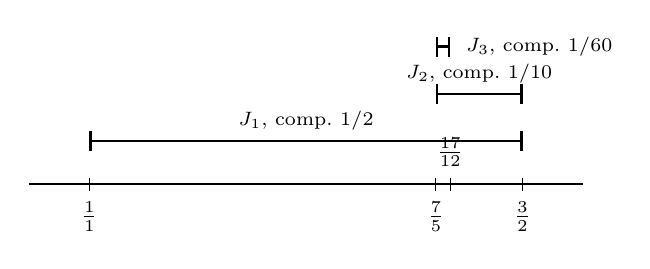
\begin{tikzpicture}[x=11cm,y=1cm]
  \draw[thick] (0.93,0) -- (1.57,0);
  \foreach \x in {1, 1.5, 1.4, 1.41667}{
    \draw (\x,0.08) -- (\x,-0.08);
  }
  \node[below] at (1,-0.1) {\small $\frac11$};
  \node[below] at (1.5,-0.1) {\small $\frac32$};
  \node[below] at (1.4,-0.1) {\small $\frac75$};
  \node[above] at (1.41667,0.1) {\small $\frac{17}{12}$};
  \draw[|-|,thick] (1,0.55) -- (1.5,0.55) node[midway,above]{\scriptsize $J_1$, comp.\ $1/2$};
  \draw[|-|,thick] (1.4,1.15) -- (1.5,1.15) node[midway,above]{\scriptsize $J_2$, comp.\ $1/10$};
  \draw[|-|,thick] (1.4,1.75) -- (1.41667,1.75) node[right,xshift=2pt]{\scriptsize $J_3$, comp.\ $1/60$};
\end{tikzpicture}
\end{center}

\begin{exemplo}
$\sqrt2 = \cf{1}{\overline{2}}$. A tabela abaixo é o produto $\Mat1\Mat2\Mat2\cdots$ lido coluna a coluna.
\begin{center}
\begin{tabular}{cccccc}
\toprule
$n$ & 0 & 1 & 2 & 3 & 4\\
\midrule
$p_n$ & 1 & 3 & 7 & 17 & 41\\
$q_n$ & 1 & 2 & 5 & 12 & 29\\
$p_n^2-2q_n^2$ & $-1$ & $1$ & $-1$ & $1$ & $-1$\\
\bottomrule
\end{tabular}
\end{center}
A última linha é o Corolário~\ref{cor:det} em ação (Pell), e $q_n/q_{n-1} = 12/5 = \cf{2}{2,2}$
ilustra o Teorema~\ref{thm:rev}.
\end{exemplo}

\subsection{O teorema de construção}

\begin{teorema}\label{thm:constr}
$(\Sig,\prec)$ é um conjunto totalmente ordenado, denso, sem extremos e \emph{completo}
(todo subconjunto não vazio limitado superiormente tem supremo). A aplicação
$\mathbf a \mapsto \bigcap_n J_n$ é um isomorfismo de ordem de $\Sig$ sobre $\R$, que leva as
palavras finitas em $\Q$ e as infinitas em $\R\setminus\Q$. Restrita às palavras infinitas, é
um homeomorfismo $\Z\times\Z_{\geq1}^{\N} \to \R\setminus\Q$ (o espaço de Baire).
\end{teorema}

\begin{proof}[Esboço]
Totalidade e densidade são imediatas da definição de $\prec$. Para a completude, dado
$S\subset\Sig$ não vazio e limitado, constrói-se o supremo \emph{letra a letra}: escolhe-se
$s_0 = \sup\{a_0 : \mathbf a \in S\}$ (finito pela limitação), depois, entre os elementos de $S$
que realizam $s_0$, escolhe-se $s_1$ como o \emph{ínfimo} dos $a_1$ (a orientação inverte),
e assim por diante; se o processo estaciona obtém-se uma palavra finita, senão uma infinita.
Verifica-se que a palavra resultante é cota superior e é $\preceq$ qualquer outra.
Que a aplicação para $\R$ é bem definida e injetiva é a Proposição~\ref{prop:encaixe} mais o
princípio dos intervalos encaixados; a sobrejetividade é o algoritmo da Seção 3.1.
A afirmação topológica segue de que os cilindros $[a_0,\dots,a_n]$ são exatamente os traços dos
intervalos $J_n$ nos irracionais, e formam base de abertos com diâmetro $\to 0$.
\end{proof}

\begin{obs}[o preço e o prêmio]
Se quisermos usar o Teorema~\ref{thm:constr} como \emph{definição} de $\R$ (e não como teorema
sobre um $\R$ pré-existente), a ordem e a topologia saem de graça, mas as operações de corpo
saem caras: não há fórmula razoável para as letras de $\mathbf a + \mathbf b$ em função das de
$\mathbf a$ e $\mathbf b$. Define-se $+$ e $\cdot$ por continuidade a partir de $\Q$, ou
algoritmicamente (o algoritmo de Gosper calcula $\frac{\alpha xy+\beta x+\gamma y+\delta}
{\varepsilon xy+\zeta x+\eta y+\theta}$ letra a letra, mantendo um estado $2\times2\times2$ ---
de novo matrizes). É por isso que Dedekind e Cauchy são as construções de manual: elas são
\emph{aditivamente} naturais. Em compensação, esta construção traz embutida a teoria da
aproximação, que nas outras é um teorema à parte:
\[
  \left| x - \frac{p_n}{q_n}\right| < \frac{1}{q_nq_{n+1}} < \frac{1}{q_n^2},
\]
e os $p_n/q_n$ são as \emph{melhores} aproximações racionais no sentido forte.
\end{obs}

\begin{teorema}[Serret --- a construção é $\GL_2(\Z)$-equivariante]
Dois irracionais $x,y$ têm palavras que coincidem a partir de certo índice se, e somente se,
$y = \gamma\cdot x$ para algum $\gamma\in\GL_2(\Z)$.
\end{teorema}

\noindent
Isto identifica o que a codificação realmente é: um sistema de coordenadas em $\Pj(\R)$ adaptado
à ação de $\GL_2(\Z)$. Trocar de palavra num prefixo finito $=$ agir por uma matriz inteira.

\section{Toda dimensão: a companheira e os corpos \texorpdfstring{$K_{n,m}$}{Knm}}\label{sec:dim}

A Seção~\ref{sec:constr} constrói $\R$. A pergunta seguinte é se a máquina sobe de dimensão --- e sobe, com a
mesma álgebra e uma troca só: $\Mat{a}$ dá lugar à \emph{matriz companheira} da borda. Mas a
subida tem uma condição, e a condição \textbf{falha} numa parte da família; esta seção diz onde.

\begin{definicao}[a borda de grau $n$ e a sua companheira]
Para $n\geq 2$ e $m\geq 1$, seja $\beta_{n,m}(x) = x^n - m\,x^{n-1} - 1$ e
\[
  \Comp{n}{m} \;=\;
  \begin{pmatrix}
    m & 0 & \cdots & 0 & 1\\
    1 & 0 & \cdots & 0 & 0\\
    0 & 1 & \cdots & 0 & 0\\
    \vdots & & \ddots & & \vdots\\
    0 & 0 & \cdots & 1 & 0
  \end{pmatrix} \in \mathrm{M}_n(\Z),
\]
a companheira de $\beta_{n,m}$. Para $n=2$, $\Comp{2}{m} = \Mat{m}$: \emph{o dicionário da Seção~1
é o caso $n=2$ desta definição}.
\end{definicao}

\begin{proposicao}[o determinante sobrevive]\label{prop:detn}
\begin{equation}\label{eq:detn}\det \Comp{n}{m} = (-1)^{n+1},\end{equation} logo $|\det| = 1$ e $\Comp{n}{m} \in \GL_n(\Z)$ com inversa
inteira, para todo $n$ e todo $m$.
\end{proposicao}

\begin{proof}
O determinante de uma companheira é $(-1)^n$ vezes o termo constante do polinómio, aqui $-1$.
\end{proof}

\noindent É o Corolário~\ref{cor:det} sem a hipótese $n=2$: a identidade fundamental não era um
acidente do caso plano. Verificado simbolicamente para $2\leq n\leq 6$, $m\in\{1,2\}$, junto com
$\chi_{\Comp{n}{m}} = \beta_{n,m}$.

\subsection{O que daria a ordem: a condição de Pisot, e onde ela falha}

O caso $n=2$ tinha ordem porque $\R$ tem ordem. Em dimensão $n$ seria preciso mais: que a
estrutura \emph{aponte} para um número real distinguido, isto é, que $\sigma$ seja um número de
Pisot. Metade disso é sempre verdade; a outra metade não é.

\begin{proposicao}[a parte que vale sempre]\label{prop:dominante}
Para todo $n\geq2$ e $m\geq1$, $\beta_{n,m}$ tem exatamente uma raiz $\sigma>1$, e ela é real e
simples.
\end{proposicao}

\begin{proof}
$\beta_{n,m}(1) = -m < 0$ e $\beta_{n,m}(m+1)>0$; e $\beta'_{n,m}(x) = x^{n-2}\big(nx-m(n-1)\big)>0$
para $x>1$, logo há exatamente uma travessia e ela é simples.
\end{proof}

\begin{obs}[a parte que não vale --- e uma distinção necessária]\label{obs:naopisot}
Não é verdade que as raízes restantes tenham todas módulo $<1$. Mas convém separar dois enunciados
que a palavra ``Pisot'' confunde: \emph{$\sigma$ ser um número de Pisot} é propriedade do seu
polinómio \textbf{mínimo}; \emph{$\beta_{n,m}$ ser um polinómio de Pisot} é propriedade de
$\beta$. Para $m=1$:
\begin{center}\small
\begin{tabular}{lll}
\hline
$n$ & $\sigma$ é número de Pisot & $\beta_{n,1}$ é polinómio de Pisot \\ \hline
$2,3,4$ & sim & sim \\
$5$ & \textbf{sim} (o menor que existe) & não \\
$\geq 6$ & não & não \\
\hline
\end{tabular}
\end{center}
\noindent Em $n=5$ os dois divergem, e o caso é explícito:
\[
  x^5-x^4-1 \;=\; (x^2-x+1)(x^3-x-1),
\]
e $x^2-x+1$ tem as suas duas raízes \emph{sobre} a circunferência unitária (raízes primitivas
sextas), de módulo exatamente $1$ --- logo $\beta_{5,1}$ não é polinómio de Pisot. Mas a única raiz
de módulo $>1$ é a de $x^3-x-1$, o \textbf{número plástico} $1{,}3247\ldots$, que é
\emph{o menor número de Pisot} (Siegel, 1944): o fator ciclotómico estraga a matriz, não o número.
O que interessa à dinâmica de $\Comp{5}{1}$ é a matriz --- as raízes de módulo $1$ não contraem. Para $n=6,\dots,12$ e $m=1$ o segundo maior módulo
é $1{,}0328;\ 1{,}0518;\ 1{,}0630;\ 1{,}0696;\ 1{,}0735;\ 1{,}0756;\ 1{,}0766$ --- todos $>1$.
Para $m\geq2$ a propriedade resistiu em todo o intervalo medido ($2\leq m\leq5$, $n\leq60$).
\end{obs}

\begin{conjectura}\label{conj:pisot}
Para todo $m\geq2$ e todo $n\geq2$, $\beta_{n,m}$ é polinómio de Pisot: a raiz $\sigma>1$ é real e
simples, e todas as restantes têm módulo $<1$.
\end{conjectura}

\noindent O critério de Brauer~\cite{brauer1951} não se aplica --- a sequência de coeficientes
$(m,0,\dots,0,1)$ não é decrescente ---, o que é também a razão estrutural de a linha $m=1$ falhar a
partir de $n=5$.

\begin{obs}[continuação]
\end{obs}

\begin{obs}[e a irredutibilidade também falha]\label{obs:redutivel}
$\beta_{n,1}$ é redutível sobre $\Q$ exatamente para $n\equiv 5 \pmod 6$, sempre com o fator
ciclotómico $x^2-x+1$. Isto é o \textbf{teorema de Selmer} (1956) e não uma observação de intervalo
finito; a prova cabe em três linhas: de $x^n\beta_{n,1}(1/x) = -(x^n+x-1)$ e $\zeta-1=\zeta^2$ para
$\zeta$ raiz primitiva sexta, vem $\zeta^n+\zeta-1 = \zeta^n+\zeta^2 = 0 \iff \zeta^n = \zeta^5
\iff n\equiv5\pmod6$. Logo
$\Q[x]/(\beta_{5,1})$ \textbf{não é corpo}: tem divisores de zero.
\end{obs}

\begin{corolario}[a conservação entre os níveis]\label{cor:conserva}
\[
  |\sigma| \cdot \!\!\prod_{\lambda \neq \sigma}\!\! |\lambda| \;=\; |\det \Comp{n}{m}| \;=\; 1 .
\]
\emph{O que a direção dominante expande, as restantes contraem exatamente tanto.}
\end{corolario}

\begin{obs}[por que este corolário não testa Pisot]\label{obs:naotesta}
O Corolário~\ref{cor:conserva} é consequência imediata de \eqref{eq:detn} e vale
\textbf{sempre} --- inclusive nos casos da Observação~\ref{obs:naopisot}, onde há raízes de módulo
$>1$. Um produto igual a $1$ é compatível com fatores individuais maiores que $1$. Medir a
conservação e concluir Pisot é, portanto, um \emph{non sequitur}: em $n=6$, $m=1$ o produto dá
$1{,}000000000000$ e mesmo assim o segundo módulo é $1{,}0328$. Para testar Pisot é preciso medir
o \emph{máximo} dos módulos não dominantes, não o produto de todos.
\end{obs}

\subsection{O que se constrói de facto}

\begin{teorema}[os corpos $K_{n,m}$]\label{thm:constrn}
Suponha $\beta_{n,m}$ irredutível sobre $\Q$ (o que exclui os casos da
Observação~\ref{obs:redutivel}). Então $K_{n,m} := \Q[x]/(\beta_{n,m})$ é um corpo de números de
grau $n$, a avaliação $x\mapsto\sigma$ da Proposição~\ref{prop:dominante} dá um mergulho
$\iota: K_{n,m}\hookrightarrow\R$, e a ordem induzida por $\iota$ é total e compatível com as
operações.
\end{teorema}

\begin{proof}[Esboço]
Irredutibilidade é hipótese. $\iota$ é morfismo de corpos, logo injetiva; a ordem de $\R$
restringe-se à imagem, e restrição de ordem de corpo é ordem de corpo.
\end{proof}

\begin{obs}[o nome importa: $K_{n,m}$ \textbf{não} é $\R^n$]\label{obs:naoRn}
$K_{n,m}$ é \emph{enumerável} e totalmente desconexo --- é um subcorpo de $\R$, de dimensão $n$
sobre $\Q$ e dimensão $1$ sobre si mesmo. $\R^n$ é não enumerável, conexo, e nem sequer é corpo
para $n\geq3$. Chamar $K_{n,m}$ de $\R^n$ confunde \emph{grau de extensão} com \emph{dimensão
topológica}, e faz o Teorema~\ref{thm:constrn} parecer dizer que a construção da Seção~\ref{sec:constr} sobe para
o plano, o que ele não diz.
\end{obs}

\begin{obs}[e $K_{n,m}$ é só um lado: o mergulho de Minkowski dá o $\R^n$]\label{obs:mink}
A objeção anterior é sobre o \emph{corpo}. Sobre o \emph{espaço} que ele gera a resposta é outra, e
as duas não se contradizem. Um corpo de números de grau $n$ tem exatamente $n$ mergulhos em $\C$ ---
$r_1$ reais e $r_2$ pares conjugados, $r_1 + 2r_2 = n$ --- e agrupando cada par como
$(\mathrm{Re},\mathrm{Im})$ obtém-se o \emph{mergulho de Minkowski}
\[
  \sigma : K_{n,m} \longrightarrow \R^{r_1}\times\C^{r_2} \cong \R^n ,
\]
cuja imagem é um \textbf{reticulado completo}. Isto é: $K_{n,m}$ é enumerável, e ainda assim
$K_{n,m}\otimes_\Q\R \cong \R^n$. Medido para $n\leq5$, $m\leq2$: $r_1+2r_2 = n$ e o reticulado tem
posto cheio em todos os casos.

\emph{E o corpo é só um lado.} O outro é o reticulado dual $L^{*}$ --- com a forma-traço, o
codiferente $\mathfrak d^{-1} \supseteq L$ --- e vale
$\operatorname{covol}(L)\cdot\operatorname{covol}(L^{*}) = 1$. \emph{Mas isto não é a conservação
$|\det| = 1$ deste texto:} é verdade para \textbf{qualquer} reticulado de posto cheio, por
definição de dual, e $\operatorname{covol}(L) = 2^{-r_2}\sqrt{|d_K|}$ não é $1$ em geral. Também
não faz sentido escrever $\R^n = L\oplus L^{*}$, pois ambos têm posto cheio no \emph{mesmo}
$\R^n$.
\end{obs}

\begin{obs}[o enunciado correto de ``toda dimensão'']\label{obs:naosobe}
O que de facto sobe de dimensão é a Seção~\ref{sec:constr} na sua forma topológica. O espaço de Baire satisfaz
\[
  \N^{\N} \;\cong\; (\N^{\N})^n \;\cong\; (\N^{\N})^{\N}
  \qquad\text{(homeomorfismos)},
\]
por intercalação de palavras; logo $\R\setminus\Q \cong (\R\setminus\Q)^n$ para todo $n$, inclusive
infinito. \emph{Este} é o ``preenche toda dimensão ponto a ponto''. Mas $\R\not\cong\R^n$ para
$n\geq2$ (invariância do domínio): o homeomorfismo existe precisamente porque os irracionais são
totalmente desconexos, e morre quando se repõem os racionais.
\end{obs}

\begin{obs}[a dimensão abaixo é a projeção dual da de cima --- quando é]
Quando $\sigma$ \emph{é} Pisot (Proposição~\ref{prop:dominante} mais a hipótese da
Observação~\ref{obs:naopisot}), iterar $\Comp{n}{m}$ projeta qualquer vetor sobre a direção
dominante, e o subespaço restante contrai e some: é a figura do cone e da espiral em $n$ níveis.
Fora desse regime a figura não vale --- há direções que \emph{crescem} além da dominante em
proporção, e não há sombra única para onde projetar.
\end{obs}


\section{A conversão primo $\leftrightarrow$ irracional}\label{sec:primos}

A base gerada pela borda não serve só para ordenar: ela \emph{seleciona primos}. Esta secção prova
a conversão nos dois sentidos e diz exatamente onde ela deixa de ser bijetiva.

\subsection{Do irracional para os primos: a norma}

Para $n=2$ a borda $x^2 = mx+1$ dá a norma
\[
  N(a+b\sigma) \;=\; a^2 + m\,ab - b^2 , \qquad D := \operatorname{disc}(\beta_{2,m}) = m^2+4 .
\]

\begin{teorema}[que primos a base representa]\label{thm:repr}
Seja $p$ primo ímpar, $p \nmid D$. Se $p = |N(a+b\sigma)|$ para alguns $a,b\in\Z$, então
$\left(\frac{D}{p}\right) = 1$. A recíproca vale \emph{se e só se} o número de classes de formas de
discriminante $D$ é $1$.
\end{teorema}

\begin{proof}
$(\Rightarrow)$ De $a^2+mab-b^2 = \pm p$, multiplicando por $4$ e completando o quadrado,
$(2a+mb)^2 - Db^2 = \pm4p$. Reduzindo mod $p$: $(2a+mb)^2 \equiv Db^2$. Se $p \mid b$ então
$p\mid 2a+mb$ e $p^2 \mid 4p$, absurdo; logo $b$ é invertível mod $p$ e $D \equiv
\big((2a+mb)b^{-1}\big)^2$, isto é, $D$ é resíduo quadrático.

$(\Leftarrow)$ Se $\left(\frac{D}{p}\right)=1$ então $\beta_{2,m}$ tem raiz mod $p$, logo $p$
decompõe-se em $\mathcal O_K$ e existe um ideal $\mathfrak p$ de norma $p$. Esse ideal é
\emph{principal} --- e portanto gerado por um elemento de norma $\pm p$ --- exatamente quando a sua
classe é trivial. Se $h(D)=1$ todas as classes são triviais e a recíproca vale; se $h(D)>1$, os
primos cujo ideal cai numa classe não principal são representados por \emph{outra} forma do
mesmo discriminante, não pela principal.
\end{proof}

\begin{obs}[a hipótese não é decorativa]
Para $m \leq 5$ tem-se $D \in \{5,8,13,20,29\}$, todos com $h(D)=1$, e a equivalência verifica-se
sem excepção. \textbf{Já $m=6$ dá $D=40$}, o discriminante de $\Q(\sqrt{10})$, que tem $h=2$ --- e a
equivalência falha logo em $p=3$: de $a^2+6ab-b^2=\pm3$ viria $(a+3b)^2-10b^2=\pm3$, e
$u^2 \equiv \pm3 \pmod{10}$ é impossível. Já para $D = 85$ ($h=2$, forma principal $x^2+xy-21y^2$) os primos com
$\left(\frac{85}{p}\right)=1$ até $60$ são $3,7,19,23,37,59$ --- note-se que $5$ e $17$ \emph{dividem}
$85$, logo têm símbolo $0$ e estão excluídos pela hipótese $p\nmid D$ --- ao passo que a forma
principal representa apenas $19$ e $59$: os restantes pertencem à outra classe.
\end{obs}

\begin{obs}[os convergentes são o núcleo, não os primos]
Para todo $\sigma_m$ e todo $n$, $N(p_n - q_n\sigma) = (-1)^{n+1}$: os convergentes dão
\textbf{unidades} --- mas com o \emph{sinal menos}. Note-se que $N(p_n+q_n\sigma)$ não é unidade
($1,5,11,31,79,\dots$ para $m=1$): é $p_n - q_n\sigma$ que é pequeno, ao passo que
$p_n+q_n\sigma \approx 2q_n\sigma$ cresce.
É o Corolário~\ref{cor:det} outra vez --- $\det M_n = \pm1$ é $N = \pm1$ --- e diz que a expansão
percorre o \emph{núcleo} da norma. Os primos aparecem nos outros elementos do reticulado, não na
diagonal que a régua percorre.
\end{obs}

\begin{obs}[o caso clássico: Fermat, 1640]\label{obs:fermat}
O Teorema~\ref{thm:repr} tem um antepassado ilustre. A forma $x^2+y^2$ tem discriminante $D=-4$, e
$\left(\frac{-4}{p}\right)=1 \iff \left(\frac{-1}{p}\right)=1 \iff p\equiv1\pmod 4$. Como
$h(-4)=1$, a equivalência do teorema aplica-se \emph{sem} a ressalva das classes, e o enunciado
reduz-se a
\[
  p = a^2+b^2 \iff p \equiv 1 \pmod 4 ,
\]
que é o teorema dos dois quadrados de Fermat. Verificado até $p=41$: $5=1^2+2^2$, $13=2^2+3^2$,
$17=1^2+4^2$, $29=2^2+5^2$, $37=1^2+6^2$, $41=4^2+5^2$, e nenhum $p\equiv3$ é representado. O nosso
teorema é a mesma lei, com $D$ arbitrário e a hipótese $h(D)=1$ a tornar-se necessária.
\end{obs}

\subsection{O período: o primo lido num racional}

A conversão tem um terceiro lado, e é o mais elementar dos três.

\begin{proposicao}[o período codifica o primo]\label{prop:periodo}
Sejam $p$ primo e $n$ uma base com $\gcd(n,p)=1$. A expansão de $1/p$ na base $n$ é puramente
periódica, e o seu período é $\operatorname{ord}_p(n)$, a ordem multiplicativa de $n$ módulo $p$.
Em particular o período \textbf{divide} $p-1$.
\end{proposicao}

\begin{proof}
$1/p$ tem período $k$ na base $n$ se e só se $n^k \equiv 1 \pmod p$, isto é, se e só se
$k$ é múltiplo de $\operatorname{ord}_p(n)$; o menor é a própria ordem. A divisibilidade é o
\textbf{pequeno teorema de Fermat}: de $n^{p-1}\equiv1$ vem $\operatorname{ord}_p(n)\mid p-1$.

\emph{Os dois teoremas de Fermat aparecem assim um em cada sentido da conversão}: o dos dois
quadrados (Obs.~\ref{obs:fermat}) do lado irracional~$\to$~primo, pela norma; o pequeno teorema
deste lado primo~$\to$~racional, pelo período.
\end{proof}

\begin{obs}[a base é a coordenada; o primo é o invariante]
Para $p = 19$ os períodos são $18$ na base $2$, $18$ na base $3$, $9$ na base $5$, $\mathbf 3$ na
base $7$ e $18$ na base $10$: cada régua lê um número diferente, e \emph{todos dividem $18 = p-1$}.
É a mesma figura do resto do texto --- o que muda é quem mede, o que fica é o que está a ser
medido.
\end{obs}

\noindent Juntando com o Teorema~\ref{thm:repr}, as três conversões fecham um triângulo:
o irracional seleciona primos pela norma; cada primo parte-se num ângulo pelo Frobenius; e cada
primo lê-se num racional pelo período.

\subsection{Dos primos para o irracional: o Frobenius}

No sentido inverso a informação é a fatoração de $\beta$ módulo $p$. Para $p$ não ramificado, o tipo
de fatoração é a classe de conjugação do Frobenius em $\operatorname{Gal}(L/\Q)$, com $L$ o corpo de
decomposição, e determina o ângulo pelo qual $p$ entra na base.

\begin{obs}[e as proporções são forçadas]
Pelo teorema de densidade de Chebotarev, cada classe de conjugação recebe uma fração de primos igual
ao seu tamanho relativo. Para $\beta_{3,1} = x^3-x^2-1$ (grupo $S_3$) as frações são $1/6$, $1/2$,
$1/3$; contados os primos até $20\,000$ (excluindo $31$, que ramifica) obtêm-se
$0{,}160$, $0{,}506$, $0{,}333$.
\end{obs}

\noindent \textbf{As duas direções são a mesma informação.} O irracional fixa a borda; a borda fixa
a norma e o discriminante; o discriminante decide, por resíduo quadrático, quais primos entram; e
cada primo que entra parte-se de um modo que é um ângulo. Contínuo e discreto são leituras de um
mesmo dado, e o que os converte é a norma num sentido e a redução módulo $p$ no outro.

\section{O que atravessa a passagem, e o que fica}\label{sec:passagem}

Esta secção é o eixo do texto. Tudo o que veio antes --- o dicionário, o determinante, a ordem, a
subida de dimensão --- e tudo o que vem depois --- os primos, a existência de ordem --- assenta num
único facto: \textbf{a estrutura parte-se em partes simétrica e antissimétrica, e só a simétrica
atravessa de uma dimensão para a de baixo}. A que atravessa mede; a que fica roda.

\subsection{A coordenada real é a fração \texorpdfstring{$1/n$}{1/n} do traço}\label{sec:umsobren}

\begin{proposicao}\label{prop:centro}
Para $\beta_{n,m}$ com raízes $\lambda_1,\dots,\lambda_n$, o \emph{centro} delas é
\[
  \frac1n\sum_j \lambda_j \;=\; \frac{m}{n} ,
\]
e é racional. Em unidades da soma, o centro vale $1/n$ \emph{exactamente}, para todo $m$.
\textbf{A identificação com $\operatorname{Tr}_{K/\Q}(\sigma)/n$ exige $\beta_{n,m}$ irredutível}:
em $n=5$, $m=1$ o polinómio mínimo de $\sigma$ é cúbico e $\operatorname{Tr}(\sigma) = 0 \neq m$.
E o centro não é a raiz real: em $n=2$, $m=1$ o centro é $0{,}5$ e $\sigma = 1{,}618\ldots$
\end{proposicao}

\begin{proof}
A soma das raízes é o simétrico do coeficiente de $x^{n-1}$, isto é $m$, e é racional; a média é
$m/n$. A razão entre a média e a soma é $1/n$, independentemente de $m$.
\end{proof}

\begin{obs}[nenhum metal é especial]
Em grau $2$ a fração é $1/2$ para \textbf{todo} $m$: $\tfrac{(\sigma+\sigma')/2}{\sigma+\sigma'} =
\tfrac12$. O caso $m=1$ não é excecional --- parece sê-lo apenas porque ali $\operatorname{Tr}=1$ e
o valor absoluto coincide com a fração. O mesmo vale para o fator ciclotómico $\Phi_6$, cujas raízes
têm parte real $1/2$ e traço $1$. \emph{A coordenada real é o ponto médio das raízes, e o ponto
médio está sempre a meio, por construção.}
\end{obs}

\noindent Em grau $n$ a divisão não é por dois: é \textbf{por $n$}. Verificado: o centro das raízes
dá $0{,}5$ em $n=2$, $0{,}333\ldots$ em $n=3$, $0{,}25$ em $n=4$, $0{,}2$ em $n=5$ --- e coincide
com $\operatorname{Tr}/n$ em todos os casos. \textbf{Cada dimensão divide pela sua própria ordem}, e
a direção real fica no centro de todas por ser a média.

\subsection{Em grau dois: as duas metades são o traço e o discriminante}\label{sec:metades}

O caso $n=2$ da Proposição~\ref{prop:centro} é o mais nítido, porque aí as duas partes têm nome
clássico.

Um par conjugado $\lambda,\bar\lambda$ parte-se canonicamente em duas metades, e cada uma é uma
coordenada:
\[
  \frac{\lambda+\bar\lambda}{2} \;=\; \rho\cos\theta
  \qquad\text{(simétrica)},
  \qquad\qquad
  \frac{\lambda-\bar\lambda}{2} \;=\; i\,\rho\sin\theta
  \qquad\text{(antissimétrica)} .
\]

\begin{proposicao}[as duas metades são o traço e o discriminante]\label{prop:metades}
Para $\beta_{2,m} = x^2-mx-1$ com raízes $\sigma,\sigma'$:
\[
  \frac{\sigma+\sigma'}{2} \;=\; \frac{m}{2} \;=\; \frac{\operatorname{Tr}}{2} ,
  \qquad
  (\sigma-\sigma')^2 \;=\; m^2+4 \;=\; D .
\]
\end{proposicao}

\begin{proof}
Soma e produto das raízes dão $\sigma+\sigma' = m$ e $\sigma\sigma' = -1$, donde
$(\sigma-\sigma')^2 = (\sigma+\sigma')^2 - 4\sigma\sigma' = m^2+4$.
\end{proof}

\noindent \textbf{Mas é preciso não confundir a metade com o seu quadrado.} A parte antissimétrica
é $\sigma-\sigma' = \sqrt D$, que troca de sinal sob a conjugação; $D$ é o seu \emph{quadrado} e
portanto \textbf{invariante} --- é racional, e é ele que atravessa. Dizer que ``$D$ é a metade
antissimétrica'' seria falso, e desmentiria a Secção~\ref{sec:primos}, onde é exactamente $D$ que
decide quais primos entram. A leitura correcta: a simétrica ($\operatorname{Tr}$) e o quadrado da
antissimétrica ($D$) são ambos invariantes e ambos atravessam; o que \emph{não} atravessa é
$\sqrt D$, cujo sinal depende de qual raiz se chama $\sigma$. Verificado para $m=1,\dots,5$: $(\sigma-\sigma')^2$ dá
$5,8,13,20,29$, que são $m^2+4$.

\begin{obs}[e é isto que decide o que atravessa a passagem]
No traço, a metade antissimétrica \textbf{cancela-se aos pares} --- $\lambda$ com $\bar\lambda$ ---
e sobrevive apenas a simétrica, multiplicada por dois:
\[
  \operatorname{Tr}(\sigma^k) \;=\; \underbrace{\sum_{\lambda\in\R}\lambda^k}_{\text{as raízes reais}}
  \;+\; \sum_{j}\, 2\,\rho_j^{\,k}\cos(k\theta_j) .
\]
\textbf{Metade atravessa; a outra metade fica.} \emph{A primeira soma tem $r_1$ termos, não um}:
para $n$ par, $\beta_{n,m}(0) = -1 < 0$ e $\beta \to +\infty$ em $-\infty$, logo há uma segunda raiz
real negativa que não pertence a par nenhum. Escrever só $\rho_0^k$ vale apenas quando $r_1 = 1$ ---
em $n=4$, $m=1$ o traço é $1$ e a fórmula truncada daria $1{,}819$. E a coordenada real é
precisamente o caso $\theta = 0$: $\lambda^k = \rho^k$ sem cosseno, a única que não oscila --- e
\emph{é por isso que é ela que ordena}. As restantes mudam de sinal e não podem ordenar nada.
\end{obs}

\subsection{A série polar, e a restrição que a base impõe}\label{sec:serie}

A recorrência $u_{k+n} = m\,u_{k+n-1} + u_k$ que a borda gera tem solução geral
\[
  u_k \;=\; \sum_{j} c_j \lambda_j^{\,k}
  \;=\; \underbrace{c_0\,\sigma^k}_{\text{o termo real}}
  \;+\; \sum_{j}\underbrace{\rho_j^{\,k}\big(P_j\cos k\theta_j + Q_j\sin k\theta_j\big)}_{\text{os pares conjugados, em polar}} ,
\]
com um cosseno amortecido por cada par conjugado. \emph{O termo dominante sozinho nunca é exato}:
falta-lhe sempre a parte oscilante, e como $\rho_j<1$ no regime bom o erro decai --- mas só se anula
no limite. \textbf{A igualdade converge apenas no infinito.}

\begin{obs}[mas os $c_j$ não são livres --- e a restrição é de simetria]
Escrita assim, a fórmula descreve \emph{qualquer} combinação, e quase nenhuma dá inteiros: com
$c=(1,0,0)$ obtém-se $u_1 = 1{,}4656\ldots$ Para que a sucessão viva no reticulado é preciso que os
$c_j$ sejam os \textbf{conjugados de Galois} de um mesmo $c\in K$, e nesse caso a soma é
\[
  u_k \;=\; \operatorname{Tr}_{K/\Q}\!\big(c\,\sigma^k\big) .
\]
O traço é a única forma linear \emph{simétrica} sob a ação de Galois --- e é exatamente ela que
transporta de $K$ para $\Q$. Verificado: com $c$ arbitrário os $u_k$ saem irracionais; com $c$ na
ordem $\Z[\sigma]$ saem inteiros, e $\operatorname{Tr}(1) = n$, $\operatorname{Tr}(\sigma) = m$ ---
a dimensão e o coeficiente da borda.
\end{obs}

\noindent Isto identifica o \emph{ponto de contacto} entre a dimensão $n$ e a dimensão $1$: não é
uma coordenada escolhida, é a projeção simétrica. As partes oscilantes cancelam-se aos pares
--- $\lambda$ com $\bar\lambda$ --- e o que sobrevive à passagem é o que é invariante sob todos os
mergulhos.


\subsection{A base é infinita em elementos e finita em dimensão}\label{sec:baseinf}

A família $\{1,\sigma,\sigma^2,\dots\}$ não termina, mas não é livre: a borda dobra-a de volta.

\begin{proposicao}[o fecho pela borda]\label{prop:fecho}
Para todo $k \geq n$, $\sigma^k$ é combinação \textbf{de coeficientes inteiros} de
$1,\sigma,\dots,\sigma^{n-1}$, e
\[
  K_{n,m} \;=\; \Q\cdot 1 \;\oplus\; \Q\cdot\sigma \;\oplus\;\cdots\;\oplus\; \Q\cdot\sigma^{n-1} ,
\]
soma directa de exactamente $n$ parcelas. Acrescentar potências não aumenta a dimensão.
\end{proposicao}

\begin{proof}
Indução sobre $k$. Para $k=n$ a borda dá $\sigma^n = m\sigma^{n-1}+1$. Para $k>n$, multiplicando a
hipótese por $\sigma$ e reduzindo o termo de grau $n$ pela borda, os coeficientes permanecem em
$\Z$. A soma é directa porque $\beta_{n,m}$ é o polinómio mínimo, logo não há relação de grau
$<n$.
\end{proof}

\begin{obs}[e por isso não há nada a ponderar]
Os coeficientes da redução são inteiros e nunca aparece denominador: para
$\beta_{3,1}$, as potências $\sigma^3,\dots,\sigma^8$ dão
$(1,0,1)$, $(1,1,1)$, $(1,1,2)$, $(2,1,3)$, $(3,2,4)$, $(4,3,6)$. \textbf{Em p.u. o peso já é $1$},
e a soma directa reconstrói o corpo sem escalas. Verificado: o posto de
$\{1,\sigma,\dots,\sigma^{19}\}$ é $3$, igual ao de $\{1,\sigma,\sigma^2\}$.
\end{obs}

\section{Quando existe ordem, e de onde ela vem}\label{sec:ordem}

A pergunta não é sobre $\C$. \textbf{$\C$ não tem estatuto especial nesta teoria} --- é um caso
particular, e o critério que o exclui não o menciona.

\begin{teorema}[Artin--Schreier, e o que ele diz de facto]
Um corpo admite uma ordem compatível com as operações se e só se é \emph{formalmente real}, isto é,
se $-1$ não é soma de quadrados. Para um corpo de números, isso equivale a ter pelo menos um
mergulho real, $r_1 \geq 1$.
\end{teorema}

\noindent Logo o que decide é $r_1$, e $\C$ é apenas a linha $r_1 = 0$:

\begin{center}\small
\begin{tabular}{lcl}
\hline
corpo & $r_1$ & ordenável como corpo \\ \hline
$K_{n,m}$ (a raiz dominante é real) & $\geq 1$ & \textbf{sempre} \\
$\Q(\sqrt2)$ & $2$ & sim \\
$\Q(i)$ & $0$ & não ($-1 = i^2$) \\
$\C$ & $0$ & não \\
\hline
\end{tabular}
\end{center}

\begin{obs}[a consequência para esta família, e é positiva]
$K_{n,m}$ tem \textbf{sempre} $r_1\geq1$, pela Proposição~\ref{prop:dominante}. Portanto a
construção \emph{nunca} falha aqui por falta de ordem --- o único obstáculo é a redutibilidade, que
é aritmética e está resolvida pelo teorema de Selmer. A fronteira que interessa a esta família não
é a de $\C$.
\end{obs}

\begin{obs}[e $\C$ raramente aparece sozinho]
Num corpo com $r_1\geq1$ e $r_2\geq1$ --- por exemplo $K_{3,1}$, com
$\sigma\colon K \to \R\times\C \cong \R^3$ --- as coordenadas complexas existem e \emph{não}
ordenam; quem ordena é a coordenada real. As fibras complexas acompanham a ordem sem a produzir:
são projeção, não fundação. Artin--Schreier não é contrariado, porque fala de ordenar $\C$
\emph{isoladamente}, e aqui ele nunca está isolado.
\end{obs}

\subsection{O algoritmo de Hurwitz em $\Z[i]$}

Convém separar duas perguntas que a notação tende a confundir.

\paragraph{O que generaliza: o algoritmo.} Nada nas Seções 1--3 usou a ordem de $\R$. Usamos
apenas (i) a ação de Möbius em $\Pj$, (ii) $\det\Mat{a}$ invertível no anel, e (iii) uma noção
de ``parte inteira''. Tomando $A = \Z[i]$ e como parte inteira o \emph{inteiro de Gauss mais
próximo} $\lfloor z \rceil$, obtemos as \emph{frações contínuas de Hurwitz}: $a_0 = \lfloor
z\rceil$, $z_{k+1} = 1/(z_k - a_k)$. Todos os enunciados matriciais valem \emph{ipsis litteris},
agora em $\GL_2(\Z[i])$ (o grupo de Picard):
\[
  M_n = \begin{pmatrix} p_n & p_{n-1}\\ q_n & q_{n-1}\end{pmatrix}, \qquad
  \det M_n = (-1)^{n+1}, \qquad
  M_n^{\mathsf T} = \Mat{a_n}\cdots\Mat{a_0}.
\]
Hurwitz provou que a expansão converge para todo $z\in\C$, e é finita exatamente quando
$z \in \Q(i)$.

\paragraph{Ordem em $\C$: três níveis que não devem colapsar.} A frase ``$\C$ não é ordenado''
é ambígua e, num dos três sentidos, falsa. Convém separar.

\begin{enumerate}
\item[(i)] \emph{Ordem total como conjunto: existe.} Fixe uma ordem total em $\Z[i]$ (lexicográfica
em $(\mathrm{Re},\mathrm{Im})$) e ponha a lexicográfica sobre as palavras de Hurwitz. Como a
codificação é injetiva, isso transporta uma ordem total para $\C$. Nem é preciso fração contínua:
qualquer bijeção $\C\to\R$ serve. Ordem total é barata.

\item[(ii)] \emph{Ordem de corpo: impossível.} Num corpo ordenado todo quadrado é $\geq0$; de
$-1 = i^2 \geq 0$ e $1 = 1^2 > 0$ vem contradição. Nenhuma deformação da cifra contorna isto.

\item[(iii)] \emph{Ordem equivariante: é a que a construção precisa, e some.} A ordem alternada da
Seção~\ref{sec:ord} não foi escolhida --- caiu de $\det M_n = (-1)^{n+1}$, isto é, de um \emph{sinal}. Sobre
$\R$ esse sinal é invariante topológico, porque $\pi_0(\mathrm{PGL}_2(\R)) = \Z/2$; sobre $\C$ o
determinante continua $-1$ mas $\pi_0(\mathrm{PGL}_2(\C)) = 1$, e o sinal deixa de separar
componentes. Concretamente, $\PSL_2(\R)$ preserva a separação em $\Pj(\R)=S^1$ (sinal da razão
cruzada) enquanto $\PSL_2(\C)$ é $3$-transitivo em $\Pj(\C)=S^2$ e a destrói.
\end{enumerate}

\noindent Note-se que o mesmo $-1$ carrega \emph{duas} informações e só uma atravessa: o módulo
$|\det|=1$ (conservação de área, Corolário~\ref{cor:conserva}) sobrevive em qualquer corpo; o
\emph{sinal} morre em $\C$. É essa metade perdida que era a ordem.

\paragraph{O que não generaliza: a ordem, e só ela.} Os intervalos encaixados \emph{sobrevivem}:
os análogos de $J_n$ são as regiões $M_n\cdot D$ (imagens de um disco por Möbius, logo discos ou
semiplanos), são encaixadas, e Hurwitz mostrou que os diâmetros tendem a zero --- a construção
\emph{topológica} funciona. O que falha é a ordem equivariante de (iii), e com ela o Teorema de
Serret, que era o que identificava a codificação como sistema de coordenadas adaptado a $\GL_2$.
Além disso a escolha de $\lfloor\cdot\rceil$ é arbitrária na fronteira dos quadrados unitários ---
não há análogo canónico de ``parte inteira''. Logo:
\begin{quote}
$\C$ \emph{não} se constrói por frações contínuas \emph{como corpo ordenado}. Constrói-se $\R$ como
acima e depois $\C = \R[X]/(X^2+1)$. O que a codificação matricial oferece em $\C$ é um
\emph{algoritmo}, uma \emph{topologia}, e uma \emph{geometria} --- não uma fundação ordenada.
\end{quote}

\paragraph{O que substitui a ordem: a razão cruzada.} Sobre $\R$ a razão cruzada é real e o seu
sinal dá a separação --- a ordem. Sobre $\C$ ela é complexa e o invariante que sobra é
\emph{ser real}, que geometricamente significa \textbf{concíclico}. A ordem é substituída por
geometria de círculos. E isto liga-se à dualidade: $\C^{*}\cong\R_{>0}\times S^1$ com
\[
  \widehat{\R} = \R \quad (\text{autodual: a parte da ordem}),
\]
\[
  \widehat{S^1} = \Z \quad (\text{a parte que dualiza contínuo em discreto}).
\]
O fator ordenado é autodual; o fator novo em $\C$ é o que troca contínuo por discreto sob
dualidade. Note-se que isto é uma dualidade em $\C^{*}$ (multiplicativo), \emph{não} uma ordem
em $\C$.

\paragraph{A geometria, que é o prêmio de consolação.} $\PSL_2(\R)$ é o grupo de isometrias que
preservam orientação do plano hiperbólico $\Hyp^2$, e $\PSL_2(\C)$ o do espaço hiperbólico
$\Hyp^3$, com $\Pj(\C) = \hat\C = \partial\Hyp^3$. Nessa linguagem (Series):
\begin{center}
\emph{a fração contínua de $x$ é a sequência de corte da geodésica de $\infty$ a $x$
através da tesselação de Farey.}
\end{center}
Os $a_i$ contam quantos triângulos consecutivos a geodésica atravessa ``pela esquerda'' e
``pela direita'' --- é a leitura geométrica da decomposição $M_n = R^{a_0}L^{a_1}R^{a_2}\cdots$.
Sobre $\Z[i]$, a mesma frase vale em $\Hyp^3$ com a tesselação por horosferas do grupo de Picard.

\section{De volta à projeção e à simetria}\label{sec:proj}

Fecha-se o círculo com o ponto de partida. Considere a reta $\ell_\alpha \subset \R^2$ de
inclinação $t=\tan\alpha$ e a projeção ortogonal $P_\alpha$ sobre ela. Escrevendo
$t = \cf{a_0}{a_1,a_2,\dots}$, a Proposição~\ref{prop:conv} diz que as \emph{colunas} de $M_n$
são os vetores inteiros $(q_n,p_n)$ e $(q_{n-1},p_{n-1})$, isto é, as duas direções racionais que
melhor encurralam $\ell_\alpha$, uma de cada lado (teorema de Klein: os convergentes são os
vértices dos fechos convexos dos pontos de rede de cada lado da reta --- as \emph{velas}). Logo
\[
  P_n \;=\; \frac{1}{p_n^2+q_n^2}\begin{pmatrix} q_n^2 & p_nq_n\\ p_nq_n & p_n^2\end{pmatrix}
  \;\xrightarrow[n\to\infty]{}\; P_\alpha,
\]
com erro controlado por $|t - p_n/q_n| < 1/q_n^2$.

Duas observações finais amarram os símbolos. Primeiro, o gerador $J=\begin{psmallmatrix}0&1\\1&0
\end{psmallmatrix}$ da Observação da Seção 2 é literalmente a matriz de \emph{simetria} em relação
à reta $y=x$, i.e.\ $S_\beta$ com $\beta = \pi/4$; e sua ação de Möbius é $z \mapsto 1/z$, a
inversão que gera as frações contínuas. Segundo, uma matriz de posto $1$ como
$S_\beta P_\alpha R_\theta$ fica completamente determinada por duas retas --- a imagem e o núcleo
--- e portanto se codifica por \emph{duas} frações contínuas, uma para cada inclinação. Giro,
projeção e simetria, escritos como palavras.

\section{Conclusão}\label{sec:conc}

Uma matriz por quociente parcial, e o produto delas: disso saem os convergentes (as colunas), a
identidade fundamental (o determinante é multiplicativo), a reversão da palavra (a transposição), a
ordem (o sinal do determinante) e a construção de $\R$ (os intervalos $M_n\cdot[0,\infty]$). O fio
mantém-se enquanto o objecto for $\GL_2(\Z)$ agindo em $\Pj$.

\emph{E parte-se onde deve dizer-se que se parte.} Ao subir para a companheira de grau $n$ deixa de
haver alfabeto, palavra e expansão: o que sobe é o análogo de \emph{um} irracional quadrático --- o
caso de período um --- e não da codificação. O análogo projectivo em dimensão $n$ é a acção de
$\GL_n(\Z)$ em $\mathbb P^{n-1}$, que dá os algoritmos multidimensionais de Jacobi--Perron e Brun, e não é
usado aqui.

\paragraph{O que fica em aberto.} A Conjectura~\ref{conj:pisot} --- $\beta_{n,m}$ é polinómio de
Pisot para todo $m\geq2$ --- é o único enunciado deste texto não coberto pela literatura consultada.
Verificou-se para $2\leq m\leq5$ e $n\leq60$ sem falhas. O critério clássico de
Brauer~\cite{brauer1951} não se aplica, porque a sequência de coeficientes $(m,0,\dots,0,1)$ não é
decrescente --- e é precisamente por isso que a linha $m=1$ é excepcional. Antes de qualquer
reivindicação de novidade, é obrigatório confrontar com Bertin \emph{et al.}~\cite{bertin} e com as
tabelas de Boyd.

\begin{thebibliography}{99}
\bibitem{bertin} M.-J. Bertin, A. Decomps-Guilloux, M. Grandet-Hugot, M. Pathiaux-Delefosse,
J.-P. Schreiber, \emph{Pisot and Salem Numbers}, Birkhäuser, 1992.
\bibitem{brauer1951} A. Brauer, \emph{On algebraic equations with all but one root in the interior
of the unit circle}, Math. Nachr. \textbf{4} (1951), 250--257.
\bibitem{cox} D. A. Cox, \emph{Primes of the Form $x^2+ny^2$}, 2.ª ed., Wiley, 2013.
\bibitem{frame1949} J. S. Frame, \emph{Continued fractions and matrices},
Amer. Math. Monthly \textbf{56} (1949), 98--103.
\bibitem{hardywright} G. H. Hardy, E. M. Wright, \emph{An Introduction to the Theory of Numbers},
6.ª ed., Oxford University Press, 2008.
\bibitem{hurwitz1887} A. Hurwitz, \emph{Über die Entwicklung complexer Grössen in Kettenbrüche},
Acta Math. \textbf{11} (1887--88), 187--200.
\bibitem{hurwitz1891} A. Hurwitz, \emph{Über die angenäherte Darstellung der Irrationalzahlen durch
rationale Brüche}, Math. Ann. \textbf{39} (1891), 279--284.
\bibitem{kechris} A. S. Kechris, \emph{Classical Descriptive Set Theory}, GTM 156, Springer, 1995.
\bibitem{khinchin} A. Ya. Khinchin, \emph{Continued Fractions}, University of Chicago Press, 1964.
\bibitem{klein1895} F. Klein, \emph{Über eine geometrische Auffassung der gewöhnlichen
Kettenbruchentwicklung}, Nachr. Ges. Wiss. Göttingen (1895), 357--359.
\bibitem{lam} T. Y. Lam, \emph{Introduction to Quadratic Forms over Fields}, GSM 67, AMS, 2005.
\bibitem{nakada1981} H. Nakada, \emph{Metrical theory for a class of continued fraction
transformations and their natural extensions}, Tokyo J. Math. \textbf{4} (1981), 399--426.
\bibitem{neukirch} J. Neukirch, \emph{Algebraic Number Theory}, Grundlehren 322, Springer, 1999.
\bibitem{perron} O. Perron, \emph{Die Lehre von den Kettenbrüchen}, Band I, 3.ª ed., Teubner, 1954.
\bibitem{selmer1956} E. S. Selmer, \emph{On the irreducibility of certain trinomials},
Math. Scand. \textbf{4} (1956), 287--302.
\bibitem{series1985} C. Series, \emph{The modular surface and continued fractions},
J. London Math. Soc. (2) \textbf{31} (1985), 69--80.
\bibitem{serret} J.-A. Serret, \emph{Cours d'algèbre supérieure}, tome I, Gauthier-Villars, 1877.
\bibitem{siegel1944} C. L. Siegel, \emph{Algebraic integers whose conjugates lie in the unit circle},
Duke Math. J. \textbf{11} (1944), 597--602.
\end{thebibliography}

\end{document}